% Chapter Template

\chapter{Evaluation} % Main chapter title

\label{Chapter5} % Change X to a consecutive number; for referencing this chapter elsewhere, use \ref{ChapterX}

\lhead{Chapter 5. \emph{Evaluation}} % Change X to a consecutive number; this is for the header on each page - perhaps a shortened title

%----------------------------------------------------------------------------------------
%	SECTION 1
%----------------------------------------------------------------------------------------
This chapter presents the detail of the experiments, results, analysis and discussion of results. For better understanding of the experiments a structure is created where the experiment detail, objectives,results,fairness and discussion about every experiment is explained.  The experiments are performed for three cases of baseline, collocated datanodes and collocated clusters. For every placement cases of baseline and collocated datanodes single Hadoop cluster is used to sort the generated data. The collocated cluster case was experimented using two set of six VMs ( a set of six VMs per Hadoop cluster) for all schedulers. All the experiments, consists three placement cases of baseline, collocated datanodes and collocated clusters and for each placement, all of four schedulers cases "cpt","cpf","fst" and "fsf" performance is evaluated. In total, every experiment consists twelve (12) cases for all the placement and schedulers cases. Below settings were the same for all the experiments:

\begin{itemize}
\item{ Every experiment was executed five times.}
\item{ Every VM had the same amount of Hard drive, memory and CPUs.}
\item{ For each Hadoop cluster, the workload was 25 GB of data.}
\item{ Five jobs were submitted for each Hadoop cluster, each job size is 5 GB.}
\item{ Three copy of workloads were stored on datanodes.}
\item{ Total of six VMs, one as namenode and five other acting as datanodes formed a Hadoop cluster.}

\end{itemize} 

\section{Experiment 1}

 In experiment one, we sort the generated workload using terasort, without tuning any parameter of MapReduce.  In each Hadoop cluster, a total of five (5) jobs were submitted by single user, where each job size was five (5) GB of data, in total twenty five (25) GB of data. The data were replicated three (3) times across datanodes for reliability.Single user submitted five jobs to default root queue of Hadoop scheduler.  There were no special configuration of Hadoop scheduler.\\  
 
 


\subsection{Objectives}
  
  One of the objectives of the experiment was to find out what is the default performance result for terasort workload. It means, the number of mappers and reducers are not pre-specified, and Hadoop scheduler is allowed to use arbitrary number of mappers and reducers. The experiment was designed to analyse the default behaviour of Hadoop scheduler for terasort. It is also important to see by default, which scheduler has better performance and which scheduler has better fairness in comparison to other schedulers. We also wanted to analyse how is the affect of speculative task execution (which is one of the optimizations to Hadoop scheduler)‌ on the performance of Hadoop. The experiment also addresses the impact of collocation for default terasort workload.\\
 
  As this is the first experiment set, where we did not changed any parameter, so the result of this experiment is used to see how the parameter change on the other experiments affects performance of Hadoop.\\  

 
\subsection{Results}
 
  During the experiment, we find out that by default, terasort runs with single reducer. For experiment the total number of mappers were more than forty (40+) and single reducer. It means, to complete a task , output of all mappers should wait for single reducer to become free and process the data which causes delay in overall job completion time. The figure \ref{fig:exp_1_mean} illustrates the mean values for job completion time for each scheduler and placement cases.\\
 

\begin{figure}[htbp]
  \centering
    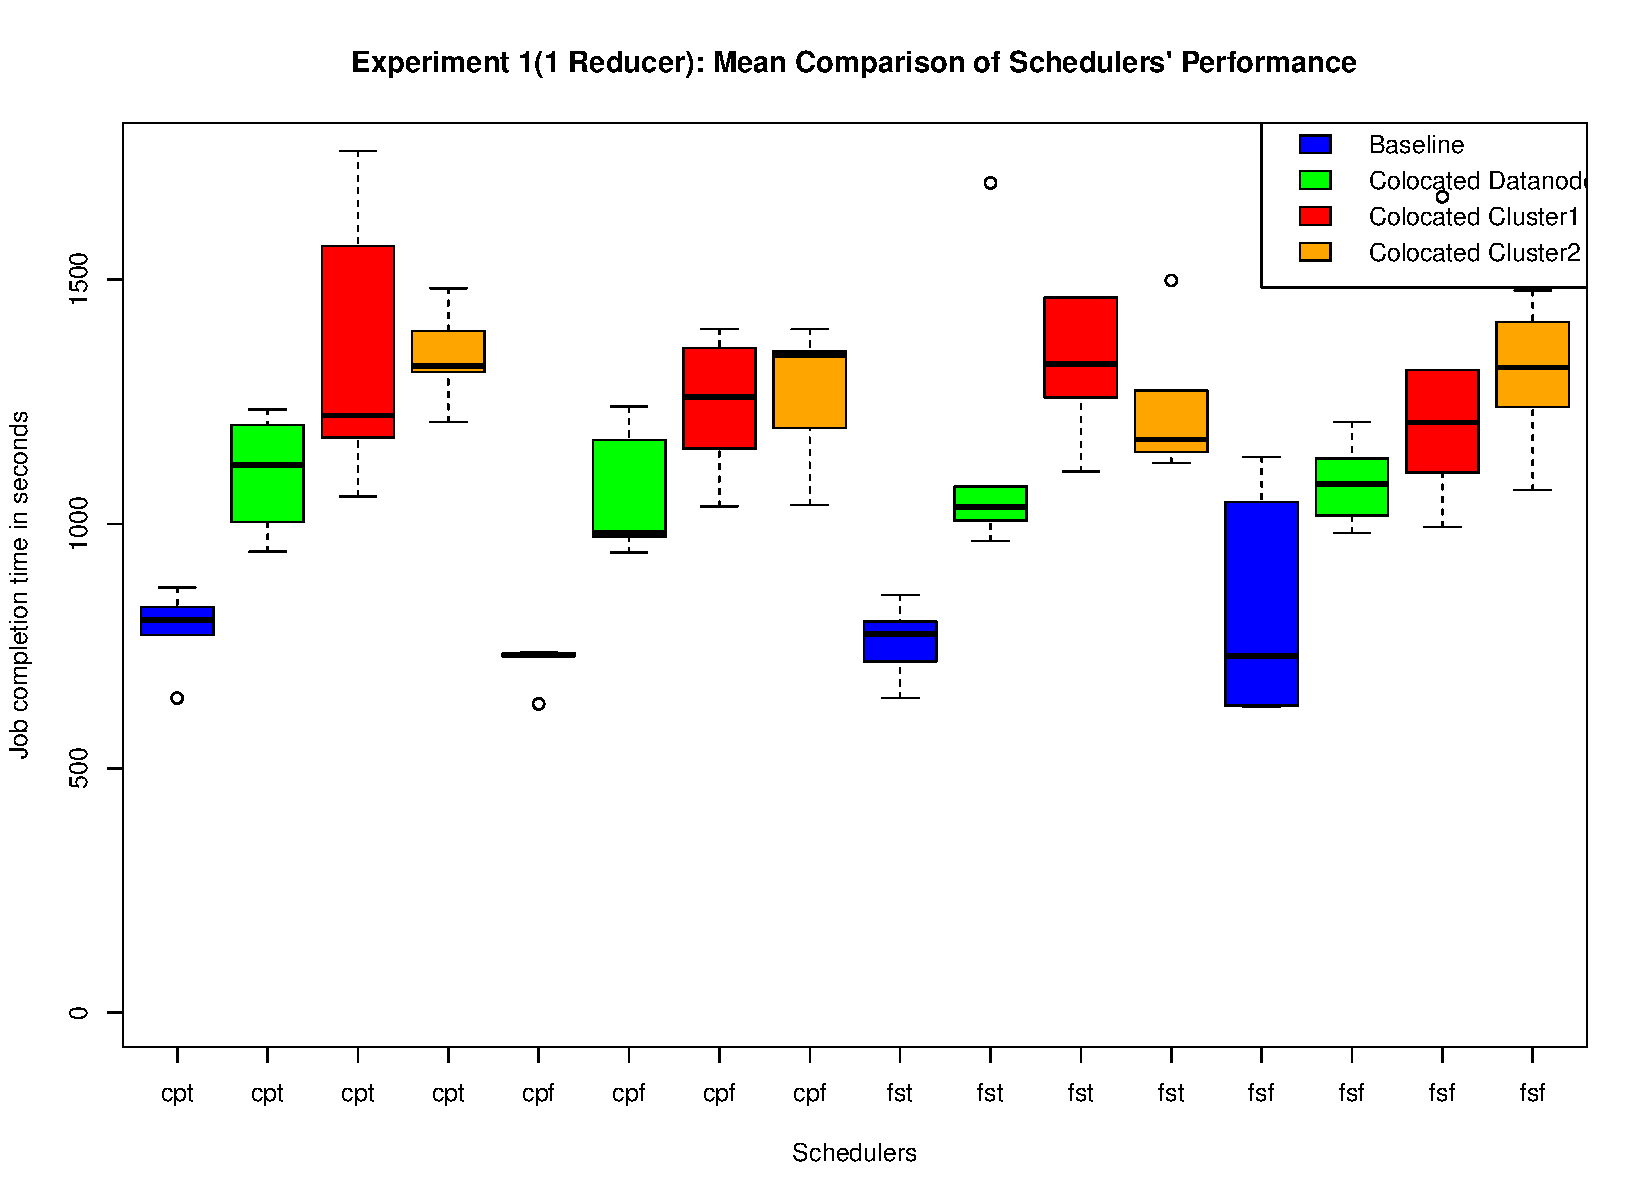
\includegraphics[width=\textwidth,height=\textheight,keepaspectratio]{./Figures/exp_1_mean.pdf}
    \rule{35em}{0.5pt}
  \caption{Experiment 1: Mean values of schedulers' performance }
  \label{fig:exp_1_mean}
\end{figure} 


\textbf{Capacity Scheduler with Speculative Task Execution (cpt)} For "cpt", the mean values of job completion time is around 850 seconds in baseline with distribution values for job completion time (performance variance) in range of 820 to 880 seconds. The mean value increases for the case of collocated datanodes to approximately 1125 seconds on average, and performance variance interval of 1000 to 1250 seconds. The collocated cluster case has the highest values for job completion ranging from 1200 to 1600 seconds with mean value of around 1400 seconds for cluster1, and range of 1340 to 1420 seconds with average of 1380 seconds for cluster2. The time difference of "cpt" performance between baseline and collocated datanodes case is 275 seconds, while the difference between baseline and collocated clusters case is higher with value of around 550 seconds.\\  

\textbf{Capacity Scheduler without Speculative Execution (cpf)} For "cpf" the mean values of scheduler performance is around 720 seconds with very small range performance variance. The collocated datanodes has the second best value for this scheduler with an average of 1125 seconds, and range of 1000 to 1250 seconds. The performance of scheduler for collocated cluster1 has an mean value of 1300 with range of 1200 to 1400 seconds, where for collocated cluster2 performance has mean value of 1310 seconds with range of 1220 to 1400 seconds. The time difference between baseline and collocated datanodes case is 405 seconds, while the collocated clusters have higher difference of 585 seconds.\\   


\textbf{Fairshare Scheduler with Speculative Execution (fst)} The "fst" scheduler has performance mean value of around 800 with range of values from 720 to 880 seconds. The collocated datanodes case has performance mean value of 1085 seconds, with range of 1050 to 1120 seconds. The performance of collocated cluster1 has mean value of 1400 seconds with range of 1320 to 1480 seconds. The performance of collocated cluster2 has mean value of around 1265 seconds with range of 1200 to 1330 seconds. The performance difference between baseline and collocated datanodes case is 285 seconds, and between baseline and collocated clusters case the difference is 630 seconds.\\ 

\textbf{Fairshare Scheduler without Speculative Execution (fsf) } The performance of "fsf" scheduler  has mean value of around 890 and range of values from 700 to 1080 seconds. The performance of "fsf" in collocated datanodes case has mean value of 1100 seconds, with range of 1020 to 1160 seconds. The "fsf" performance for collocated cluster1 has mean value of 1240 seconds for and range of values from 1120 to 1360 seconds. The "fsf" performance in collocated cluster2 case has mean value of around 1345 seconds with range of 1260 to 1430 seconds. The performance difference between baseline and collocated datanodes  case is 110 seconds, and between baseline and collocated clusters case the difference is 400 seconds.\\


\textbf{Side-Effects of Collocation} For three various node placement cases, the performance of both capacity scheduler and fairshare scheduler including the cases with and without speculative task execution are affected by collocation of datanodes. The results show that, collocation of datanodes has negative impact on performance of Hadoop schedulers and leads to longer job completion time. Though, in both collocation cases two datanodes were placed on single physical machine, but the collocated clusters case has worse results for Hadoop performance in comparison to collocated datanodes case. This is because in collocated clusters, the two nodes running on top of single machine are managed by two different namenodes, which does not know about each other, and their decisions harms the performance of collocated datanodes. It means, collocation of datanodes from different clusters does provide equal result to collocation of datanodes from the same cluster. \\  

\textbf{Speculation Effects }  For experiment one,  the speculative task execution does not improve the performance of Hadoop schedulers. Inversely, in baseline case for capacity scheduler the "cpf"‌ has better performance with mean value of 720 seconds in comparison to "cpt" which has mean value of 850 seconds. For fairshare scheduler, the "fst" has better performance compare to "fsf", in baseline,collocated datanodes and collocated clusters cases. As result for experiment 1,  the fairshare scheduler performance is improved using speculative task execution, while the capacity scheduler performance degraded by use of speculative task execution.   





\subsection{Fairness }

The figure \ref{fig:exp_1_max-min} illustrates the fairness of job completion time for all the schedulers. The figure \ref{fig:exp_1_max-min} shows that "fst" scheduler has the smallest range of values for job completion time in comparison to all other schedulers in baseline. For collocated datanodes and collocated clusters cases, the results of fairness is not well distinguishable, this is because, the number of reducers used in this experiment is only one, which means, results of the mappers should wait for single reducer for further process, thus, fairness is lost for almost all the cases of schedulers and placement cases.    

 \begin{figure}[htbp]
  \centering
    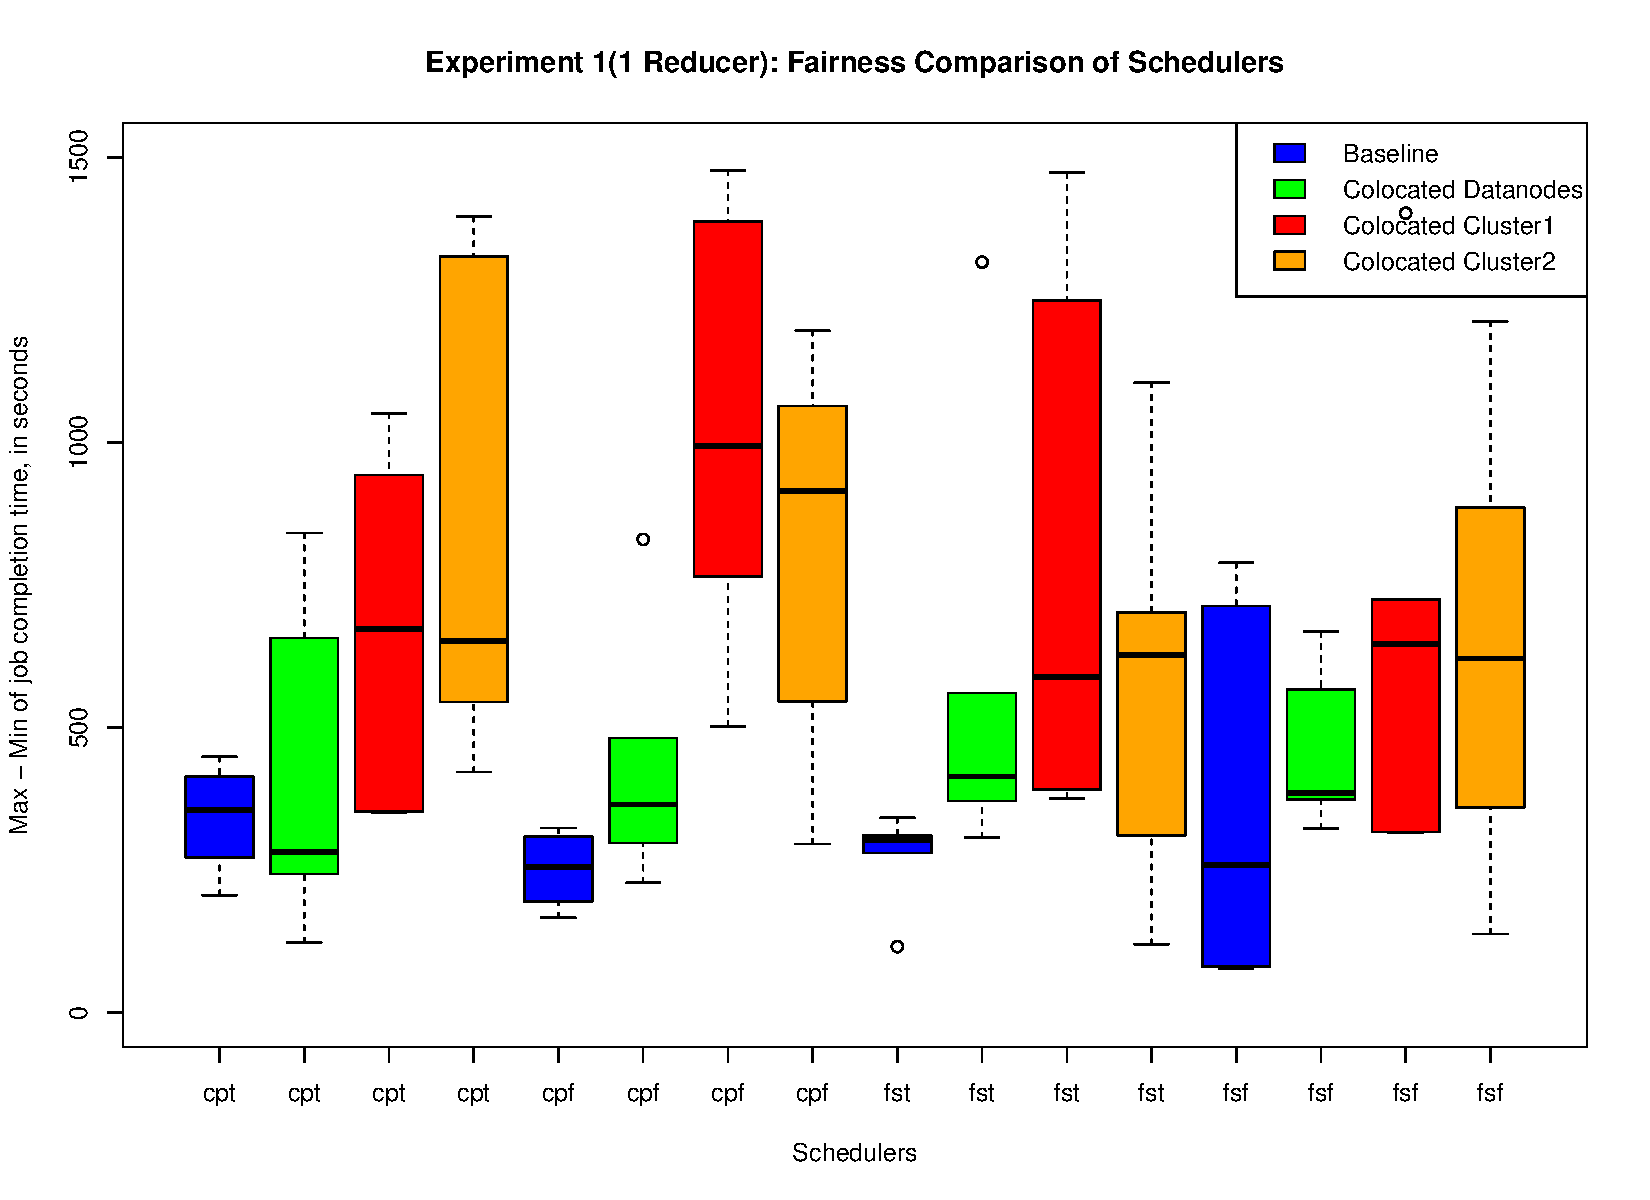
\includegraphics[width=\textwidth,height=\textheight,keepaspectratio]{./Figures/exp_1_max-min.pdf}
    \rule{35em}{0.5pt}
  \caption{Experiment 1: Fairness comparison of schedulers' performance }
  \label{fig:exp_1_max-min}
\end{figure} 
  

\subsection{Discussion}

There is single reducer used by terasort to complete the sort function for all mappers. If the reducer is used to process the output of a mapper, the output of other mappers should wait till the reducer become free. Waiting for reducer to redirect the output of mapper causes noticeable delay on performance of Hadoop schedulers. Thus, the results of experiment one, does not reflect clear distinguishable different values for the performance of capacity and fairshare schedulers. The philosophy behind fairshare scheduler is to provide fairness for all the jobs submitted.  The delay caused by single reducer to process output of mappers causes that, fairshare scheduler also does not have very vivid fairness in experiment one. The performance of schedulers for cases of speculative task execution and non speculative task execution are also affected almost equally by single reducer, thus, it makes it hard to judge from results of experiment one, that speculation leads to better performance of Hadoop scheduler. \\ 

The results explained for experiment one shows that, the collocation of datanodes either from same or different clusters leads to longer job completion time or performance degradation of Hadoop. Running two datanodes from the same cluster ( collocated datanodes case)‌ has better performance in compare to two datanodes from different clusters. It means, the side effects of a datanodes from different clusters is higher than side effects of datanodes from same cluster, and this is true for all the schedulers. \\  
  




 


%-----------------------------------
%	SUBSECTION 1
%-----------------------------------
\section{Experiment 2}

In experiment 2, single user submits five jobs to schedulers in all sub cases of experiment. Each job consists five GB‌ of data generated by Teragen (total of 25 GB data) and need to be sorted by terasort using Hadoop. Three copy of data were replicated and stored using HDFS‌ across datanodes of Hadoop cluster. There is no queue configuration for Hadoop schedulers and default root queue is  used for submission of all jobs. We changed (in contrast to experiment 1) the settings of experiment two and configured 10 reducers to participate in data processing. ‌ 




\subsection{Objectives}

As explained in discussion part of experiment one, single reducer causes considerable delay in job completion time for all Hadoop schedulers. The objective of experiment 2 is to see how the number of reducers has affect on job completion time or performance of Hadoop. In experiment two, by increasing the number of reducers to ten, our expectation was to have better performance evaluation in comparison to experiment one. It is also important, to see how the performance of Hadoop is improved by increased number of reducers for collocated datanodes and collocated clusters. 



\subsection{Results}
The figure \ref{fig:exp_2_mean} illustrates the mean value results for all the experiment cases. Over all , the job completion time is better than experiment one, it means number of reducers have important role in Hadoop performance.\\

\begin{figure}[htbp]
  \centering
    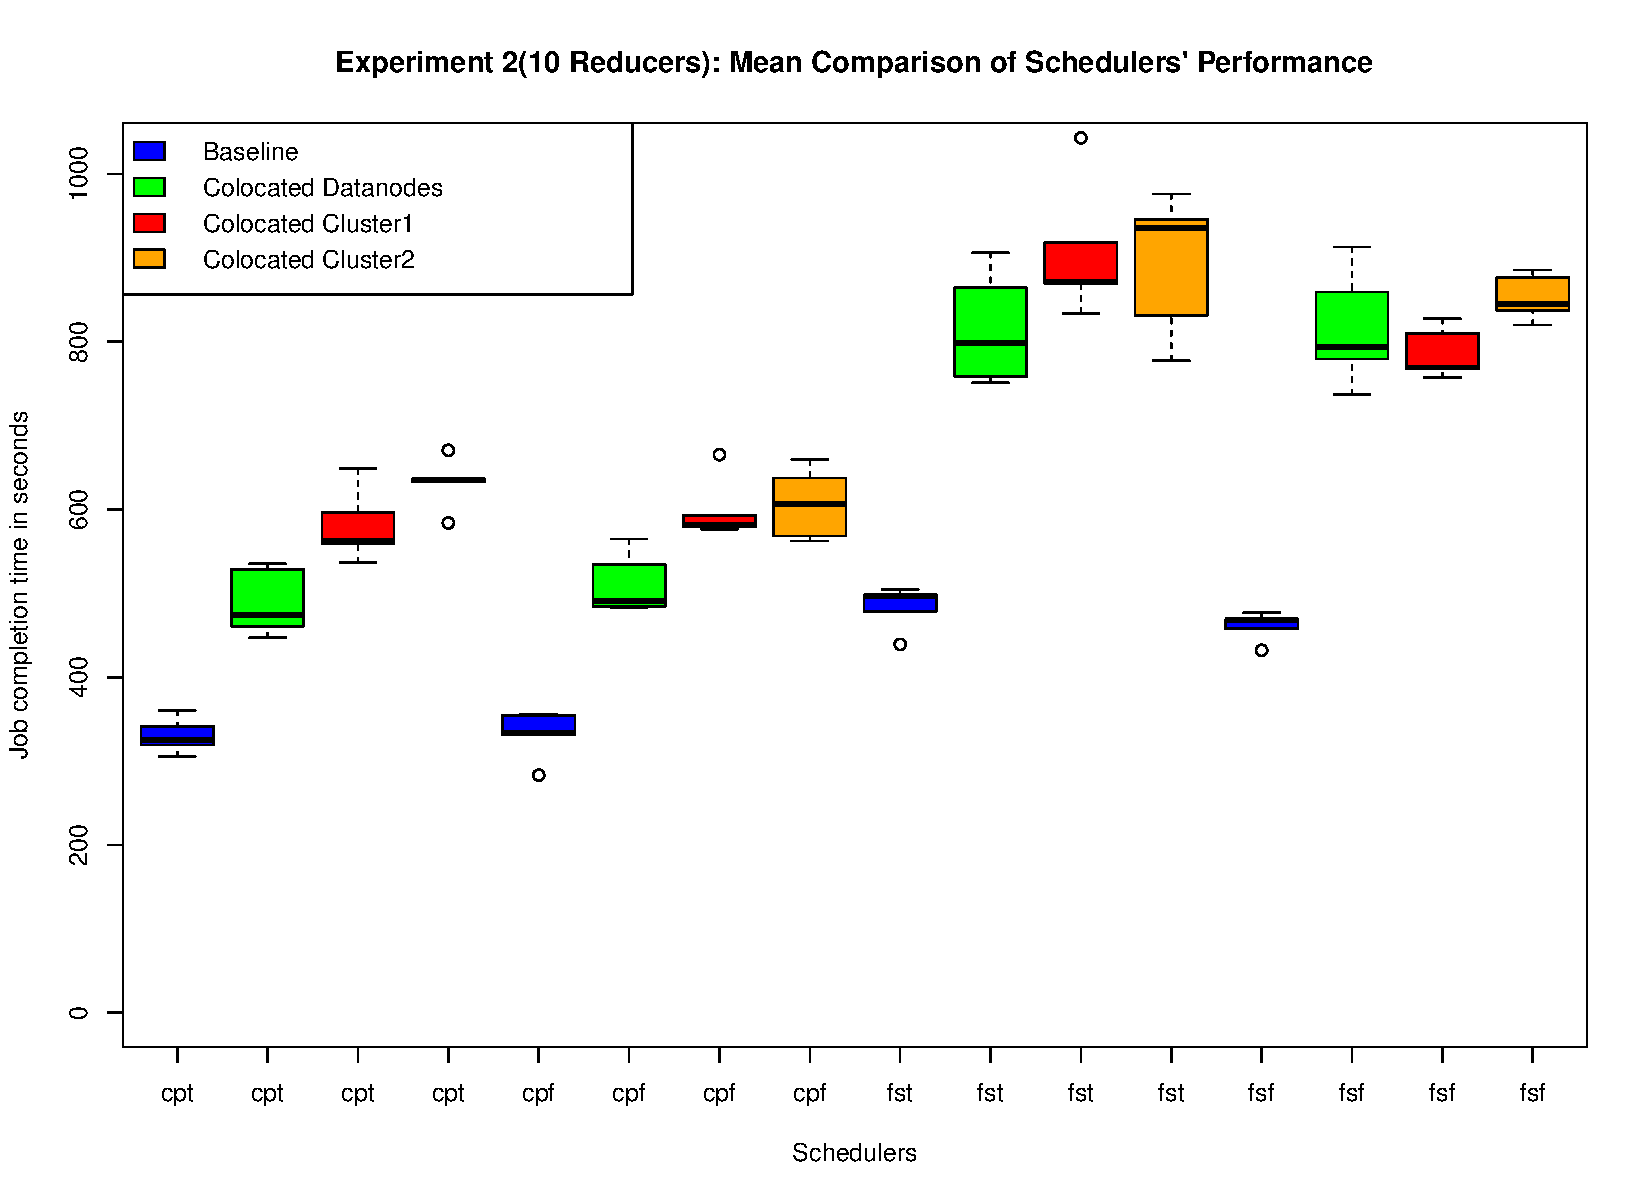
\includegraphics[width=\textwidth,height=\textheight,keepaspectratio]{./Figures/exp_2_mean.pdf}
    \rule{35em}{0.5pt}
  \caption{Mean value of schedulers' performance }
  \label{fig:exp_2_mean}
\end{figure} 

\textbf{Capacity Scheduler with Speculative Execution (cpt)} The mean value for "cpt" performance in baseline case is approximately 300 seconds, which is the best value among all schedulers cases. For collocated datanodes, the scheduler performance has mean value of approximately 500 seconds, which shows that collocation of datanodes increased the job completion time 70\% more than the baseline. For collocated clusters cases, the scheduler performance has mean value of approximately 600 seconds (approximate average for both clusters), which is double value of job completion time in comparison to baseline and shows 100\% increment job completion time.\\

\textbf{Capacity Scheduler without Speculative Execution (cpf)}  The mean value for "cpf" performance  in baseline case is approximately 330 seconds, which is worse than "cpt" ( which was 300 seconds), but the second best result among all the schedulers. The side effects for collocated datanodes case of "cpf" is almost similar to "cpt". The collocation of datanodes has an average performance of approximately 530 seconds for job completion time, which shows 70\% increment in job completion time in comparison to baseline. The average performance for collocated clusters is approximately 600 seconds for both clusters, which shows 95\% increment in job completion time. \\


\textbf{Fairshare Scheduler with Speculative Execution (fst)} The mean value for "fst" performance in  baseline case is approximately 500 seconds, which is the worst mean value among all schedulers' performance. The "fst" performance in collocated datanodes case has mean value of around 800 seconds, which shows 60\% increment and time difference of 300 seconds for job completion time in comparison to baseline. The "fst" performance in collocation of datanodes case from different Hadoop clusters has mean value of around 900 seconds, which shows 80\% increment (400 seconds time difference of job completion time) in comparison to baseline case.\\

\textbf{Fairshare Scheduler without Speculative Execution (fsf) } The  mean value for "fsf" performance  in baseline case is approximately 480 seconds, which is better than "fst" and third best value among all the schedulers. The "fsf" performance in collocation of datanodes case has mean value of approximately 800 seconds for job completion time, which shows 66\% increment and 320 seconds time different in comparison to baseline case. The "fsf" performance in collocated datanodes case from different clusters,  has mean value of around 800 seconds ( approximate value for both clusters), which is the same result as collocated datanodes case in comparison to baseline. \\


\textbf{Side-Effects of Collocations } The results in figure \ref{fig:exp_2_mean} show, that fairshare scheduler has worse performance for the collocation cases in comparison to capacity share scheduler. The mean value difference between baseline and collocated datanodes for "fst", which shows the side effects of collocation, is around 300 seconds, while this value is around 200 seconds for "cpt" case. Also, the mean value difference between baseline and collocated clusters cases, for "fst" is 400 seconds, while this value is 300 seconds in "cpt" case.\\ 

For cases, where tasks are executed by schedulers without speculation (like "cpf" and "fsf" cases), still , capacity share scheduler has better performance for collocation cases in comparison to fairshare scheduler. The mean value difference for between baseline and collocated datanodes for "cpf" is 200 seconds, which is better than the mean value difference of 320 seconds for "fsf" case. The mean value difference between baseline and collocated clusters cases for "cpf" is 270 seconds, for which "fsf" has higher difference of 320 seconds. 


\textbf{Speculation Effects } By having a deeper look to mean values in figure \ref{fig:exp_2_mean}, it is evident that speculative task execution improved the performance of capacity share scheduler ( see the "cpt" case), while decreased the performance of fairshare scheduler. Though the performance improvement of speculative task execution is minor, but still the improvement for "cpt"‌ is consistent and true for the collocated cases in comparison to "cpf" case. In contrast to capacity share scheduler, the  fairshare scheduler with speculative task execution, in "fst" case has worse result in comparison to "fsf" case. \\  ‌  


 \subsection{Fairness}
 The figure \ref{fig:exp_2_max-min} illustrates the fairness for job completion time, among submitted jobs for each placement and scheduler cases. The results show that overall fairshare scheduler has much better fairness in comparison to capacity share scheduler. The fairness for job completion time ranges from around 50 to 200 seconds for all the placement cases of fairshare scheduler, while the results for capacity share scheduler ranges from 200 to 400 seconds.\\ 
 
 
 
  For "cpt" in baseline case, the fairness values for job completion time is in the interval of 210 to 260 seconds, which shows at least 210 seconds difference. While for both "cpt" and "cpf" in baseline case, the fairness values is lower than 300 seconds on average, the collocation had negative impact and increases the fairness values to higher than 300 seconds, and even close to 400 seconds for collocated datanodes case of "cpt".
 
 
 \begin{figure}[htbp]
  \centering
    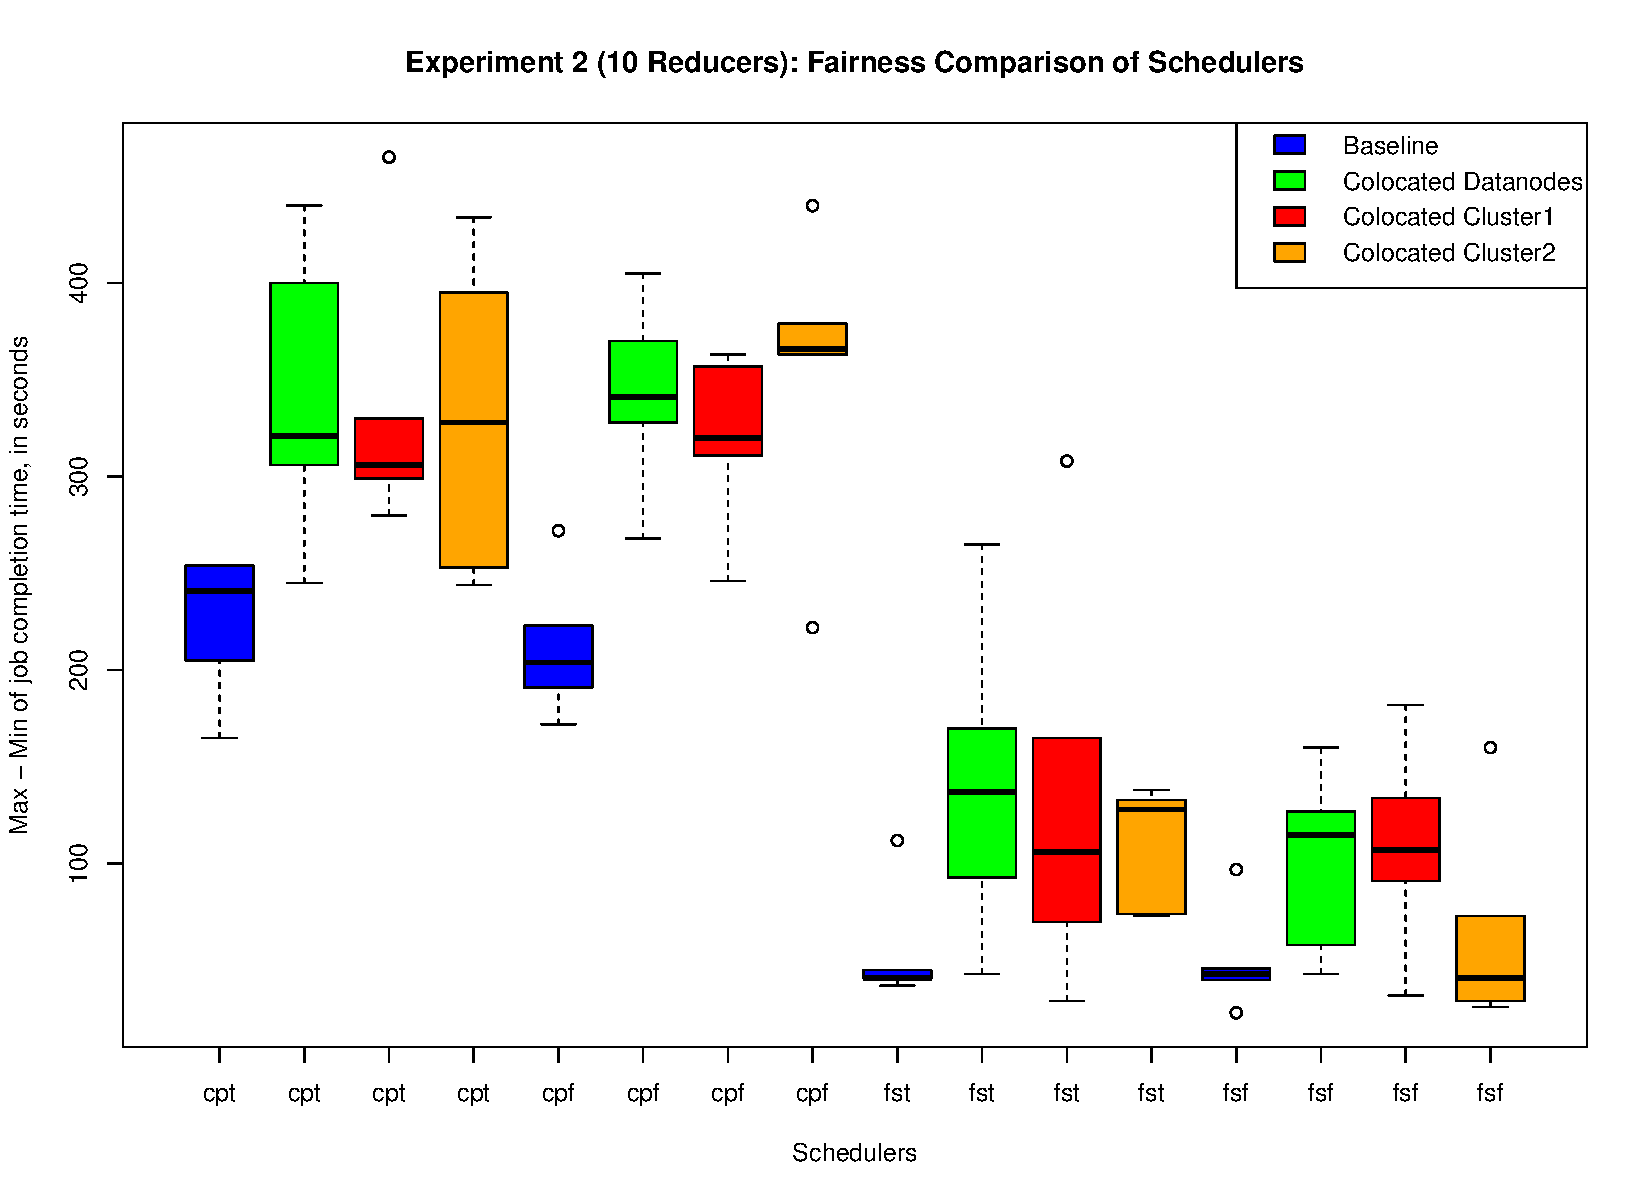
\includegraphics[width=\textwidth,height=\textheight,keepaspectratio]{./Figures/exp_2_max-min.pdf}
    \rule{35em}{0.5pt}
  \caption{Experiment 2: Fairness comparison of schedulers' performance }
  \label{fig:exp_2_max-min}
\end{figure} 
  

\subsection{Discussion}

By increasing the number of reducers from one ( in experiment one) to ten ( in experiment two ), we see that the performance of Hadoop schedulers are improved for all the cases. Which means, for process of workload using Hadoop, the selection of fair number of reducers plays a key role on performance of Hadoop. The number of mappers were consistent for all the schedulers, it was 40 mappers. In case of speculation of schedulers, some tasks were speculatively executed, which added speculative number of mappers and reducers. \\


The results shown for experiment two, indicates that capacity share scheduler has better performance in comparison to fairshare scheduler, and executes the submitted jobs in smaller time interval than fairshare schedulers. The performance of capacity share schedulers is better than fairshare schedulers in both cases of speculative and non speculative task execution, and all collocation cases.\\

The collocation cases have impact on schedulers performance and degrades the performance of Hadoop schedulers. The side effects of collocation for fairshare schedulers are higher than capacity share. The side effects of collocated datanodes is not as much as collocated clusters. This is because, in collocated datanodes, both nodes are controlled by single namenode,which mean, namenode is aware of the status of namenode using resources manager. In collocated clusters cases, the collocated datanodes are belong to separate namenodes that are not aware of status of collocated datanode, so the performance of datanode from cluster one effects the performance of datanode of cluster two.\\  
 

 The fairshare schedulers provide better fairness performance for submitted jobs. Considering the performance evaluation of and fairness evaluation of schedulers, the fairness has cost for fairshare schedulers and that causes performance degradation of Hadoop. One may use capacity share to have better performance and fairshare scheduler to guarantee better fairness for job process.\\



%-----------------------------------
%	SUBSECTION 2
%-----------------------------------

\section{Experiment 3}
The results from experiment two show that increasing the number of reducers improves the performance of Hadoop. In experiment three, we increased the number of reducer to twenty (20) reducers, which is 50\% of the number of used mappers. Rest of the experiment settings were the same as experiment one and two, where single users submitted five jobs, each job consist of five GB of data. There were no special queue configuration for Hadoop schedulers. The experiment was executed for all the placement cases and schedulers cases. 
  
\subsection{Objective}
The objective of the experiment was to find out the effects of increased number of reducers on performance of Hadoop schedulers. The side-effects of collocation and evaluation of performance improvement for the schedulers were the other objectives. The improvement of fairness for schedulers and  performance improvement of schedulers by speculative task execution were the other expected outcome of the experiment. 

\subsection{Results }
By increasing the number of reducers to 20 reducers, the evaluation shows that performance of Hadoop is increased across all the schedulers. While the effect of changing the number of reducer for experiment to experiment two was very vivid and clear, the effect of changing the number of reducers from ten to twenty in experiment three is not so high in comparison to experiment two. This means, that having so many reducers does not improve the performance of Hadoop and we may select a fair number schedulers (25\% to 50\% of mappers limited to our experiment environment and settings) for Hadoop. The figure \ref{fig:exp_3_mean} illustrates the mean values of job completion time for schedulers in all the placement cases.  


\begin{figure}[htbp]
  \centering
    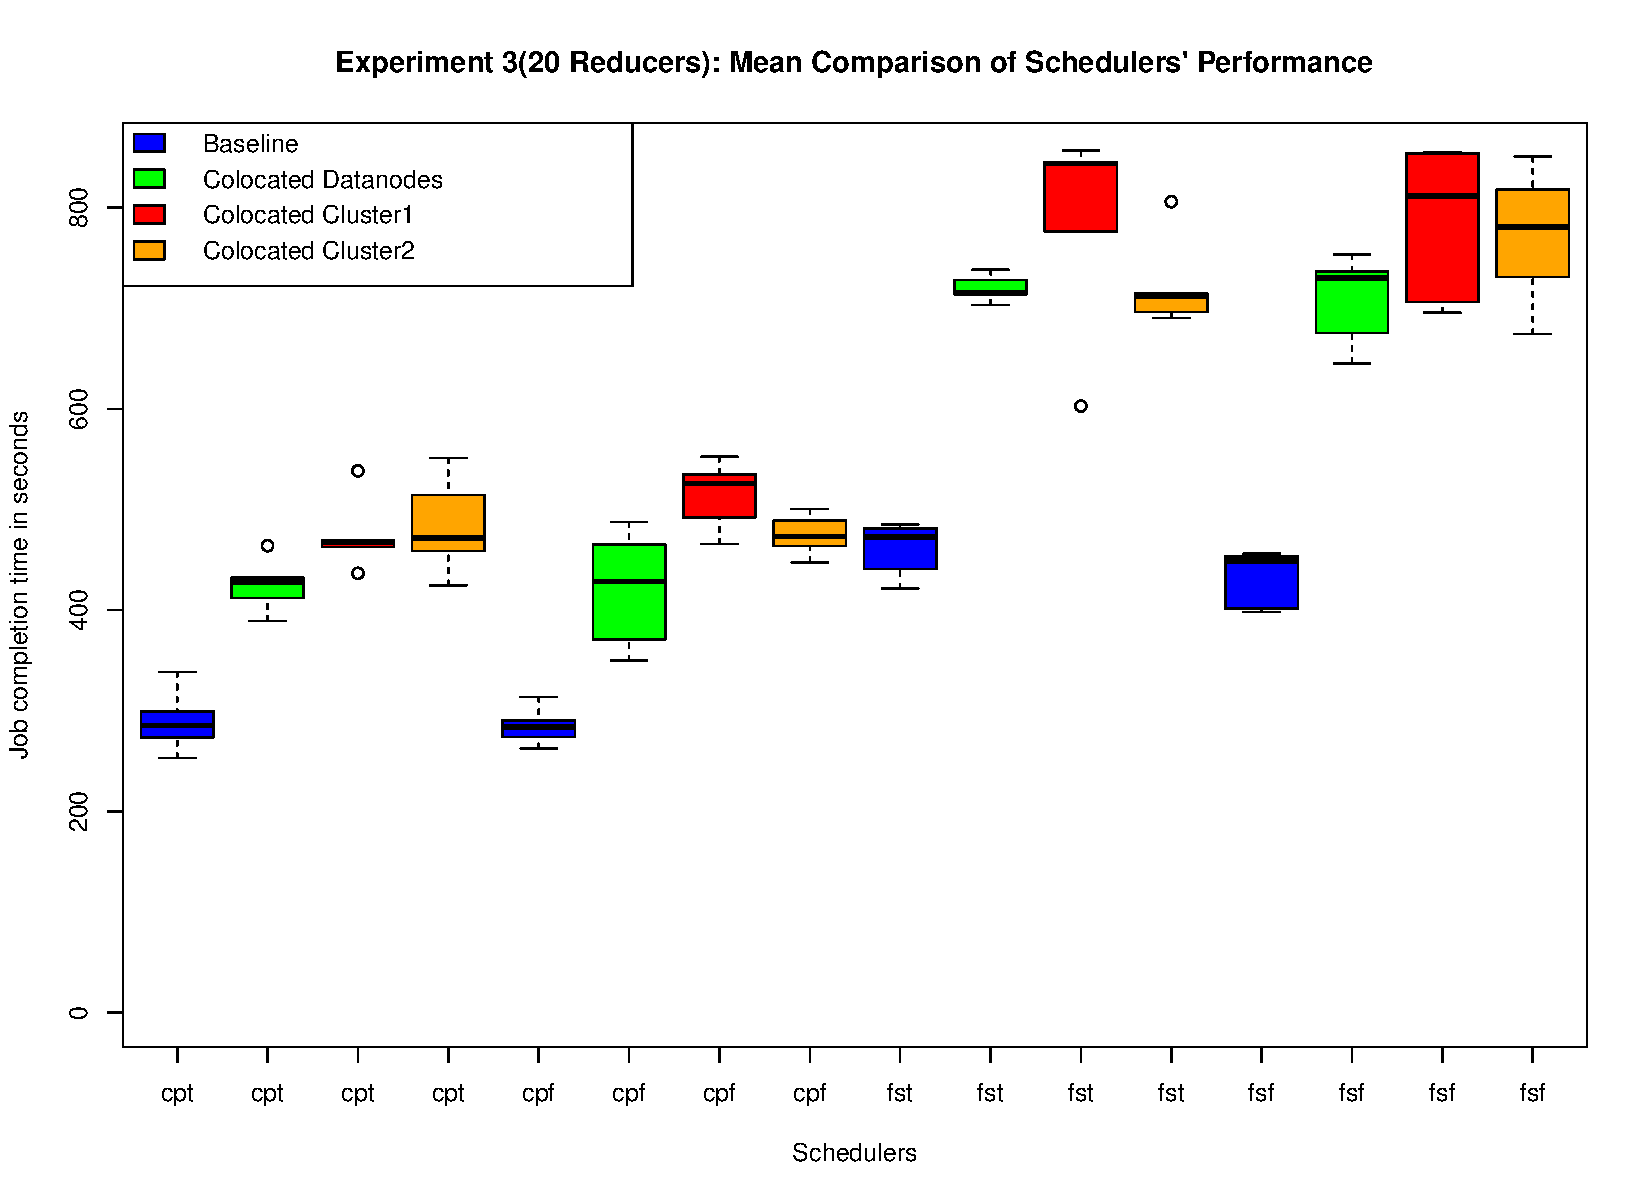
\includegraphics[width=\textwidth,height=\textheight,keepaspectratio]{./Figures/exp_3_mean.pdf}
    \rule{35em}{0.5pt}
  \caption{Experiment 3: Mean value of schedulers' performance}
  \label{fig:exp_3_mean}
\end{figure}


\textbf{Capacity Scheduler with Speculative Execution (cpt)} The mean value for "cpt" performance in baseline case is approximately 290 seconds. For collocated datanodes, the scheduler has mean value of approximately 420 seconds for job completion time, which shows that collocation of datanodes increased the job completion time 45\% more than the baseline. For collocated clusters case, the scheduler has job completion time of approximately 500 seconds (approximate average for both clusters), which has time difference of 210 seconds in comparison to baseline and shows 72\% increment in job completion time.\\

\textbf{Capacity Scheduler without Speculative Execution (cpf)} The mean value for "cpf" performance  in baseline case is approximately 290 seconds, which is same as "cpt", but the distribution range of job completion time is smaller in comparison to "cpt" . The effects of datanodes collocation on median job completion time in the "cpf" case is similar to "cpt", but the job completion time is scattered in larger interval of time. The collocation of datanodes has an average of approximately 430 seconds for job completion time, which shows 48\% increment in job completion time in comparison to baseline. The average job completion time for collocated clusters is approximately 520 seconds for both clusters, which shows 79\% increment in job completion time. \\ 


\textbf{Fairshare Scheduler with Speculative Execution (fst)} The mean value for "fst" performance in  baseline case is approximately 470 seconds, which is the worst mean value among all schedulers' performance in baseline. The collocated datanodes, has performance with mean value of around 710 seconds, which shows around 51\% increment and time difference of 240 seconds for job completion time in comparison to baseline. The collocation of datanodes from different Hadoop clusters are very different, cluster1 has a mean value of around 800 seconds, and cluster2 has mean value of 700 seconds. The mean value for both clusters is around 750 seconds,  which shows around 60\% increment with 280 seconds time difference of job completion time in comparison to baseline.\\

\textbf{Fairshare Scheduler without Speculative Execution (fsf) } The  mean value for "fsf" performance  in baseline case is approximately 430 seconds, which is better than "fst" and third best value among all schedulers. The collocation of datanodes, has mean value of approximately 700 seconds for job completion time, which shows around 63\% increment and 270 seconds time different in comparison to baseline. The collocated datanodes from different clusters have mean value of around 750 seconds ( approximate value for both clusters), which shows around 74\% increment with time difference of 320 seconds for job completion time in comparison to baseline. \\
 ‌  
\textbf{Node Placement Effects } Similar to experiment two, the side effects of collocation for both collocated datanodes and collocated cluster cases is high for fairshare scheduler in comparison to capacity share scheduler. For capacity schedulers the mean value of baseline in comparison to collocated datanodes and collocated clusters cases show the respectively time difference values of 135 and 220 seconds. While, for similar comparison the fairshare schedulers have time difference values of 255 and 300 seconds. \\    

 Across all the schedulers, the mean values for collocated datanodes is lower than mean value for collocated clusters. This proofs the fact, that collocation of datanodes from same cluster has less side effects on collocated datanode in comparison to collocation of datanodes from different schedulers.\\  



\textbf{Speculation Effects }  The illustrated results in figure \ref{fig:exp_3_mean} shows that the speculative task execution does not improve the performance of schedulers in all the cases. For "fst" in baseline case, the speculative task execution leads to worst result in comparison to "fsf". The comparison of mean values for "cpt" and "cpf" shows that there are no vivid performance improvement between speculative and non speculative task execution in all the placement cases. \\ 

 

\subsection{Fairness}
 The figure \ref{fig:exp_3_max-min} illustrates the fairness for job completion time, among submitted jobs for each placement and scheduler cases. As the results show, the fairshare schedulers have  values  lower than 250 seconds, in contrast , the fairness values for capacity share schedulers are higher than 250 seconds. The "fsf" scheduler has the best fairness value of 50 seconds, with small range of of distribution for job completion time. The fairness values shown for fairshare schedulers in collocated cases indicates that, collocation of datanodes has negative impact on fairness of schedulers, and leads to larger range for job completion time.\\ 
 
 The results shown for capacity share schedulers in all the placement cases explains, that they have higher value of 250 to 500 seconds. Both collocation cases (collocated datanodes and collocated clusters) have almost similar fairness values with mean of around 450 seconds for almost both "cpt" and "cpf", while "cpf" has larger range values for job completion time.  
 
 
  

\begin{figure}[htbp]
  \centering
    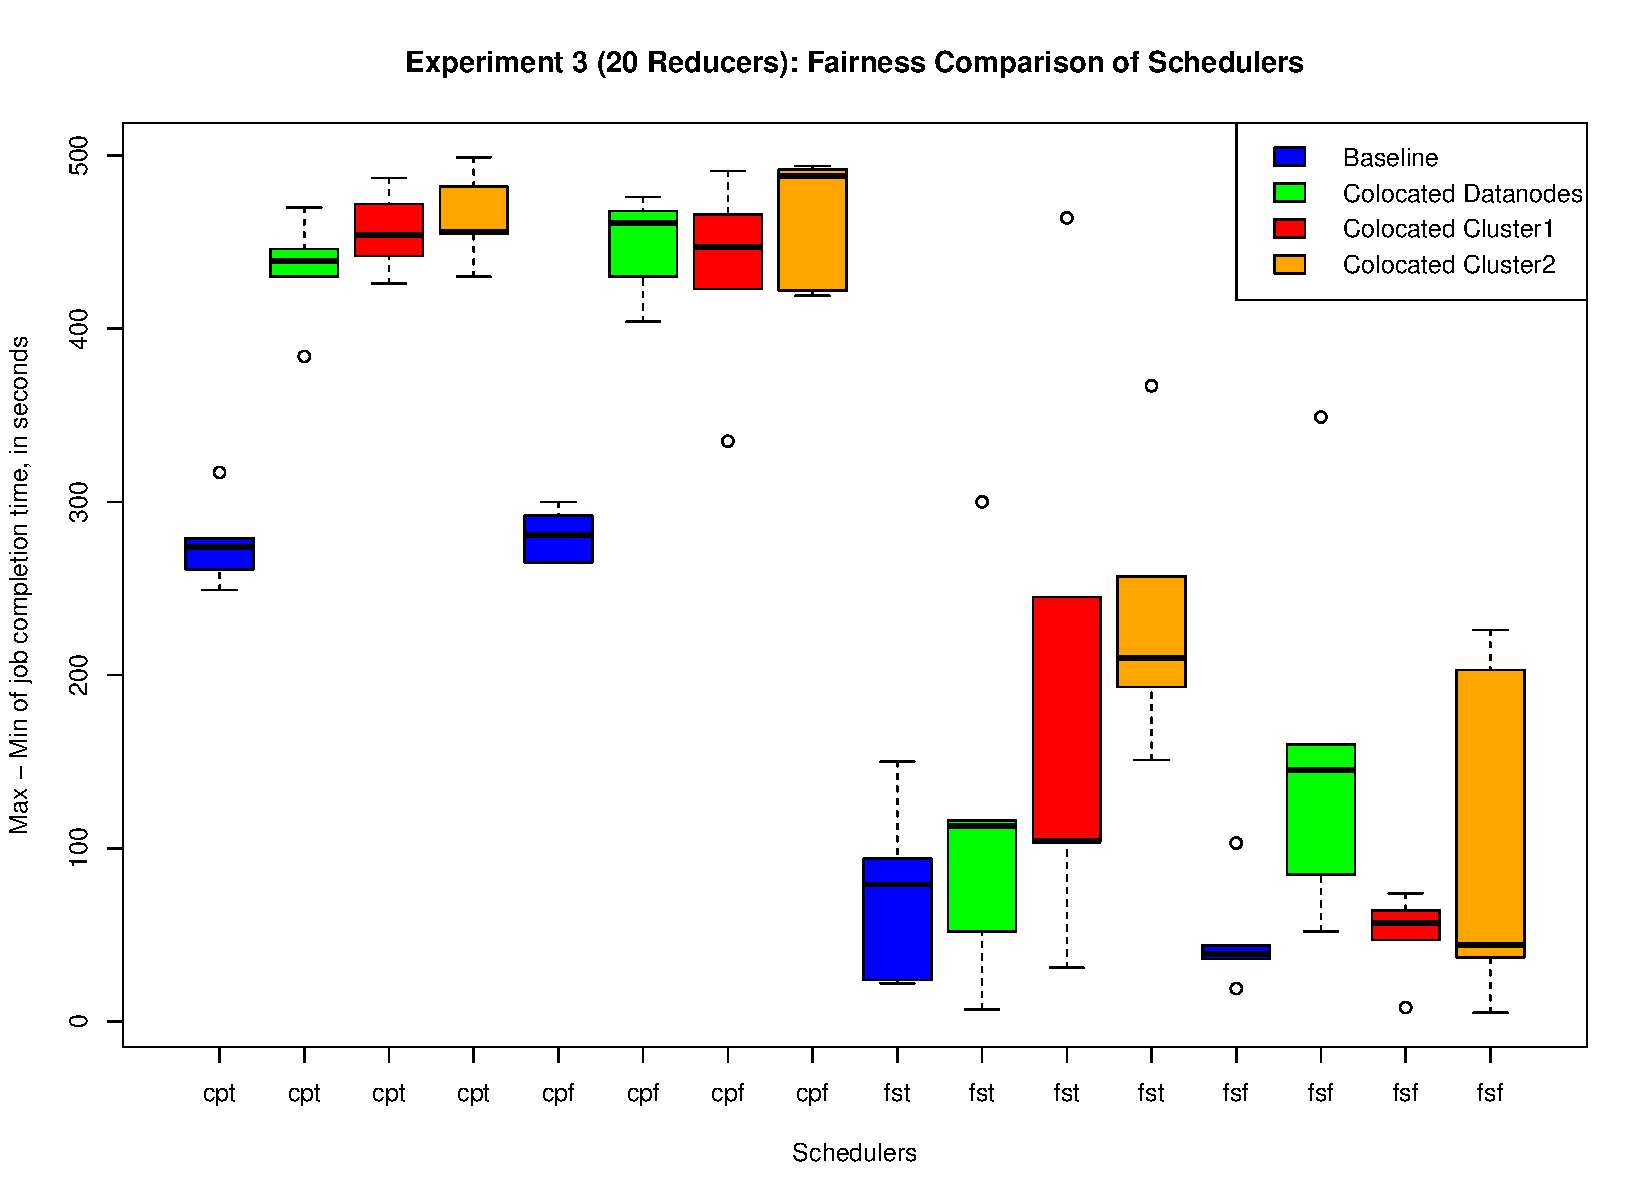
\includegraphics[width=\textwidth,height=\textheight,keepaspectratio]{./Figures/exp_3_max-min.pdf}
    \rule{35em}{0.5pt}
  \caption{Experiment 3: Fairness comparison of schedulers' performance }
  \label{fig:exp_3_max-min}
\end{figure}

\subsection{Discussion}
Though increasing the number of reducer lead to better performance in experiment two, in experiment three by increasing the number of reducers to twenty, which is 50\% of mappers (total of 40 mappers were used), the performance improvement is not so much. It means, selection of high number of reducers does not improve the performance of Hadoop, and we must select a fair number of reducers. The results from all three experiments (experiment one, two and three) for which the number of reducers were respectively 2.5\%, 25\% and 50\% of mappers, the experiment three had best results for all the schedulers in all the cases.\\


In regard to performance evaluation of schedulers, in one hand, the capacity share scheduler has the best results for both "cpt" and "cpf" cases. on the other hand, the capacity scheduler has worst fairness results in comparison to fairshare scheduler. Inversely, the fairshare scheduler has the worst performance for job completion and best fairness values in comparison to capacity share scheduler. \\

Similar to two previous experiments, the collocation cases have negative impact on performance of schedulers. In comparison to fairshare scheduler, the capacity share scheduler has more tolerance to collocation of datanodes in both cases of collocated datanodes and collocated clusters and has better performance. The capacity share scheduler also have minor better performance while speculatively executing the tasks, while in fairshare scheduler the speculative task execution causes minor degradation to the performance of scheduler.  \\  
 

 


%----------------------------------------------------------------------------------------
%	SECTION 2
%----------------------------------------------------------------------------------------

